\documentclass[output=paper]{LSP/langsci} 
\ChapterDOI{10.5281/zenodo.1090958}
\author{Moritz Schaeffer\affiliation{Johannes Gutenberg University of Mainz}\lastand Michael Carl\affiliation{Renmin University of China}}
\title{Language processing and translation} 
\label{schaeffer-carl}
%\epigram{Change epigram in chapters/01.tex or remove it there }
\abstract{The current chapter reviews studies which investigate the behavioural differences during reading and writing for translation and other non-translational language use. This chapter further argues that eye movement measures imported from Psychology are not well suited to describe the unique co-occurrence of reading and writing during written translation. In order to address these shortcomings, one existing measure (the Eye-Key Span,  \citealt{Dragsted2008,Dragsted2010}), which describes how reading and writing activities are coordinated, is further tested by replicating existing findings with more language combinations and participants. A second, novel measure (the probability that source text reading and target text writing overlap in time) is used in conjunction with the Eye-Key Span to test predictions from an existing model of the translation process \citep{Schaeffer2013Shared}. Finally, one new feature (HCross) is introduced with which an existing model of bilingual memory \citep{Hartsuiker2004} is extended.}
\maketitle

\begin{document}

\section{Translation and non-translational language processing} 
There is a long tradition of studying the differences between original texts written in one language and texts translated from a different language -- in terms of the product of translation, i.e., in corpora of the final (published) texts \citep[e.g.][]{476033}. Corpus-based translation studies have the great advantage that the data which led to the formulation of theoretical insights is ecologically valid to a high degree: the texts used in corpora such as the CroCo corpus \citep{476033} are published texts and have therefore been produced in situations which are real and natural. Experimental studies, on the other hand, often manipulate source texts (henceforth ST) and the STs are normally far shorter than those in real life situations (ranging from single words, to single sentences and short texts of approximately 150 words). In addition to the unnatural characteristics of the STs, participants are often not allowed to use reference material such as dictionaries or glossaries and typically do not have access to the internet. Further increasing the unnatural conditions of experimental studies is the fact that participants translate knowing that their reaction times or keystrokes and\slash or eye movements are recorded and the simple presence of a researcher may further impinge on the process of translation. However, the shortcoming of corpus-based translation studies is that it is difficult to attribute observed effects to particular aspects of the translation \textit{process}, given that the source of information is typically the frequency of a particular item in the \textit{final product}. The factors which led to the observed result of the process remain hidden in the dialogue between ST reading and target text (henceforth TT) reading and writing and interaction with other information sources.

The current study therefore aims to provide insights into the cognitive processes which occur during translation by first reviewing existing studies which compare translational and non-translational language use and by comparing the effect of two tasks (monolingual copying and translation) on two behavioural measures. One of these behavioural measures was first proposed by \citet{Dragsted2008} and \citet{Dragsted2010}, and the second behavioural measure is novel. The two measures take into account both eye movements on the source text and typing activity. The \isi{eye-key span} \citep{Dragsted2008,Dragsted2010} describes the temporal distance between a first reading of a particular word and the first keystroke which contributed to the translation of that particular ST word. It can be seen as a relatively late indicator: Many intervening processes between a first reading and the first keystroke can and typically do occur during translation, while fewer occur during monolingual copying. The second measure is the probability that ST reading and TT typing occur (at least partially) at the same time. It is an indicator of \isi{cognitive effort}: the less likely the co-occurrence of these two processes, the more effortful the process. The more likely it is that reading and writing overlap in time, the less effortful is the process as a whole at that time. These two measures take into account one aspect of the nature of the \isi{translation process} which it shares with few other tasks, apart from monolingual copying: the direct relationship between read input and written output.

\largerpage
Jakobsen argued that with the introduction of eye tracking and keylogging into translation \isi{process research} the hope was that
\begin{quote}
\ldots eye data would provide evidence pertaining identifiably to source-\isi{text reading} so that source-text comprehension processes could be studied separately from text-production processes and could be compared with other reading processes that were not part of a \isi{translation process}. \citep[41]{Hild2011}
\end{quote}
Very few studies have systematically compared the cognitive processes during non-translational language use with those that occur during translation. The current chapter will review the studies which have done so and will provide new evidence which addresses shortcomings in existing studies.

\section{Reaction times and eye movements during translation}
\subsection{Reaction times per clause}

\citet{Shreve1993} compared reading times in three tasks and groups: reading for later translation by translation students, reading for later monolingual paraphrasing by students of English and reading for comprehension by students in psychology. Reading times were measured per clause (including re-reading) and normalised by the number of words in each clause. Results from principal component analysis of the reading times showed that, at least on the basis of these behavioural measures, none of the four factors of the principal component analysis distinguished reading for translation clearly from the other two tasks. However, reading for translation was overall more similar to reading for monolingual paraphrasing than to reading for comprehension. The authors further point out that there was more variation in how translators read for translation while the other two groups of participants approached their tasks more homogeneously. The paraphrasing and translation groups were also asked to indicate post-task the nature and number of problems in the clauses they identified in their reading. The expectation was that the number of problems identified post-task would correlate with reading times. This was not the case. Although the authors do not interpret their findings in this way, it is entirely possible to argue that post-task identification of problems might not accurately reflect the processes which occurred during reading, given that they are produced off-line. One other reason might be the fact that reading times per clause might not accurately reflect actual reading times, which might show the expected effect locally rather than globally.

\subsection{Reaction times per word}
\largerpage
In a series of studies, Bajo and colleagues \citep{Macizo2004a, Macizo2006b,Ruiz2008Activation} employed more sensitive behavioural measures, i.e., reaction times per word using the self-paced reading paradigm. In all three studies, a similar experimental design was used: masked self-paced reading is the sequential presentation of single words which is controlled via button press by the participant, so that subsequent button presses are used to measure reaction times per word. The interval between two successive button presses is taken as an indication of the time needed to process the currently displayed word. These studies therefore address the concerns raised in relation to the study by \citet{Shreve1993}. Bajo and colleagues \citep{Macizo2004a, Macizo2006b,Ruiz2008Activation} refer to the model proposed by \citet{Seleskovitch1976} who argued that translation is normally carried out sequentially in that the first step is source text comprehension and only when this is complete and only once the source material is ``deverbalised'' can reformulation in the \isi{target language} begin. Opposed to this sequential view is the assumption that representations specific to the \isi{target language} (TL) are activated at the same time as \isi{source language} (SL) representations are activated (horizontally and in parallel). The vertical model by \citet{Seleskovitch1976} is essentially what in \isi{machine translation} would be called an interlingual model. It is the highest level in the Vauquois triangle \citep{Vauquois1968} (see \figref{schaeffer-carl:fig:1}), where transfer occurs at a language-independent interlingual representation, common to all languages.

\begin{figure}
\resizebox{.7\textwidth}{!}{
    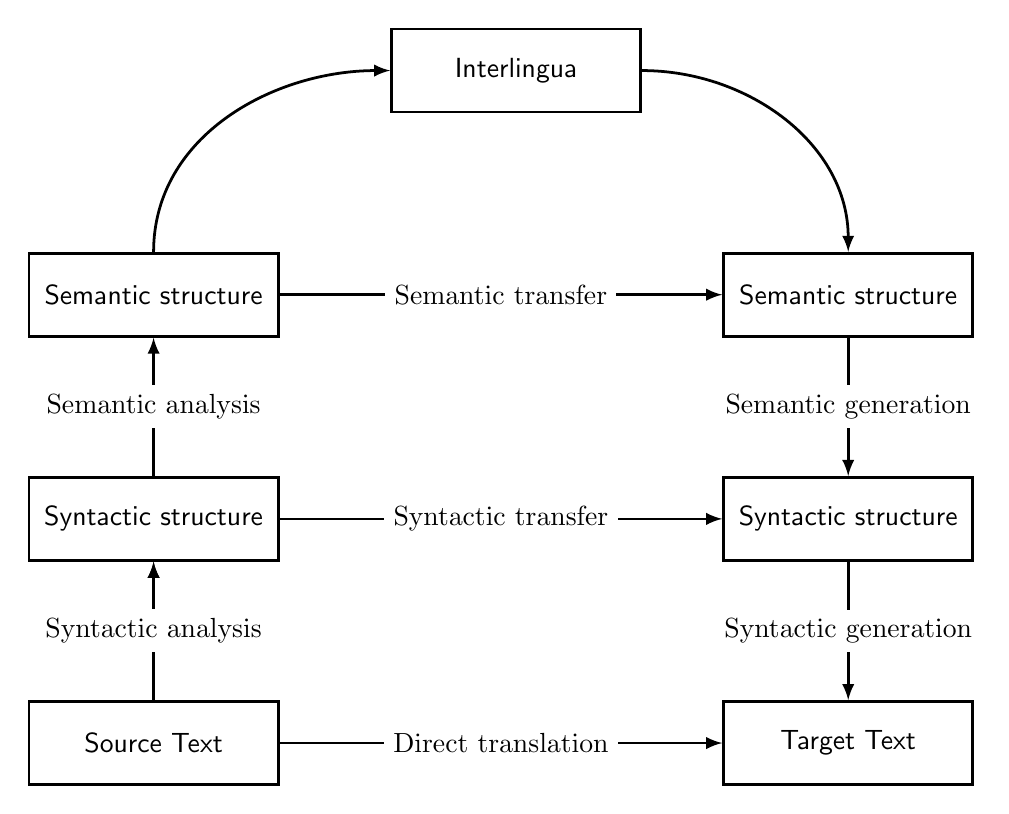
\begin{tikzpicture}
    \usetikzlibrary{shapes,arrows,positioning}
    % Styles
        \tikzstyle{block} = [rectangle, draw, fill=white, text centered, minimum height=3em, minimum width = 9em, line width = 0.1em]
        \tikzstyle{line} = [draw, -latex, line width=0.1em]
    % Place nodes
        \node [block] (source) {\sffamily{Source Text}};
        \node [block, above=5em of source] (syntactic1) {\sffamily{Syntactic structure}};
        \node [block, above=5em of syntactic1] (semantic1) {\sffamily{Semantic structure}};

        \node [block, above right = 5em and 4em of semantic1] (interlingua) {\sffamily{Interlingua}};

        \node [block, right=16em of source] (target) {\sffamily{Target Text}};
        \node [block, above=5em of target] (syntactic2) {\sffamily{Syntactic structure}};
        \node [block, above=5em of syntactic2] (semantic2) {\sffamily{Semantic structure}};

    % Label
        \draw[line] (source) -- (syntactic1) node [midway, fill=white] {Syntactic analysis};
        \draw[line] (syntactic1) -- (semantic1) node [midway, fill=white] {Semantic analysis};
        \draw[line] (source) -- (syntactic1) node [midway, fill=white] {Syntactic analysis};
        \draw[line] (semantic1.north) to[out=90, in=180] (interlingua.west);

        \draw[line] (interlingua.east) to[out=0, in=90] (semantic2.north);
        \draw[line] (semantic2) -- (syntactic2) node [midway, fill=white] {Semantic generation};
        \draw[line] (syntactic2) -- (target) node [midway, fill=white] {Syntactic generation};

        \draw[line] (source) -- (target) node [midway, fill=white] {Direct translation};
        \draw[line] (syntactic1) -- (syntactic2) node [midway, fill=white] {Syntactic transfer};
        \draw[line] (semantic1) -- (semantic2) node [midway, fill=white] {Semantic transfer};
    \end{tikzpicture}
}
%\fbox{\includegraphics[width=\textwidth]{figures/schaeffer-carl/Vauquois.png}}
\caption{The Vauquois triangle of translation based on \citet{Vauquois1968}}
\label{schaeffer-carl:fig:1}

\end{figure}

The studies by Bajo and colleagues were designed to test the Seleskovitch model. Participants in all three studies carried out two tasks: reading for comprehension and reading for translation. Participants were not overtly producing the translation while reading --
\largerpage
they were asked to orally produce the translation after having read the sentence (for translation). The expectation in all three studies was that the manipulation of the stimuli would elicit an effect only in the reading for translation condition, because of a) increased working memory load due to the added effort related to online translation and b) because the assumption was that during reading for comprehension the TL would not be activated and TL-specific manipulations would not have an effect on source text (ST) reading. In the 2004 study, Macizo and Bajo manipulated both working memory load and the availability of pragmatic cues. The stimuli consisted of object relative sentences such as ``The judge that the reporter interviewed dismissed the charge at the end of the hearing.'' The authors argued that working memory load would be particularly high for the verbs of the main clause and the relative clauses, because in object relative clauses, the thematic roles of the first two constituents (\textit{judge} and \textit{reporter} in the example) can only be assigned retrospectively once the subordinate verb (\textit{interviewed}) is read. Pragmatic cues consisted of verbs which were either more or less predictable based on the previous context. It is, for example, more predictable that a reporter interviews than that a reporter admires or it is more predictable that a judge dismisses a charge than that he drives a car.

In addition to testing the sequential versus parallel view of translation, \citet{Macizo2004a} tested the predictions of the Revised Hierarchical Model (RHM) of bilingual memory \citep{Kroll1994} which predicts that backward translation (BT, from L2 into L1) is faster than forward translation (FT, from L1 into L2), because L2 lexical representations have stronger connections to their L1 equivalents than to shared conceptual representations. Translation from L2 into L1 is therefore predicted to use the faster lexical routes and translation from L1 into L2 is mediated by the less direct conceptual connections. However, during translation, both routes are always activated -- one is simply faster than the other. The predictions based on the sequential/parallel model and the RHM are therefore that an effect appears only in the reading for translation condition and that FT, because it is more conceptually mediated than BT, is especially susceptible to the manipulation of pragmatic cues. These results are clearly borne out by the evidence: Reaction times were significantly slower during reading for translation, particularly during FT and particularly for the constructions which require retrospective assignment of thematic roles and therefore high working memory load, supporting the parallel activation of SL and TL representations during reading for translation. In addition, more predictable verbs were read significantly faster than less predictable verbs in FT, but not in BT, supporting the predictions of the RHM.

Further support for the \isi{co-activation} of SL and TL representations during reading for translation was provided by the two subsequent studies \citep{Macizo2006b,Ruiz2008Activation}. In both studies, participants also read single sentences for comprehension and for translation in a self-paced reading paradigm. In the 2006 study, the stimuli for experiments 1a and b consisted of interlingual homographs which created an ambiguity only if they were translated: the \ili{Spanish} word \textit{presente} is not ambiguous in \ili{Spanish} (it can only refer to the present time), but it is ambiguous when translated into English, given that \textit{present} can refer both to a gift and the present time. In experiment 1a and b, the number of words intervening between the ambiguous homograph and the disambiguating context was manipulated so that working memory load was a factor in the design. In experiment 2a and b, cognates were used. The manipulation in experiments 1a and b was expected to result in inhibition only when the reading purpose was translation and particularly when the working memory load was high, but not when the reading purpose was comprehension alone. The prediction for experiment 2a and b was that the presence of cognates would facilitate. Both of these predictions were designed to lend further support to the hypothesis that activation of the TL during ST reading is task-dependent. Again, the predictions were confirmed in this study. The 2004 study by Macizo and Bajo only employed professional translators, but the 2006 study by the same authors replicated the effects found in professional translators with innocent \isi{bilinguals} who had no professional translation experience: interlingual homographs, the working memory manipulation and cognates resulted in the same pattern of results, suggesting that the mechanisms underlying the task-dependent \isi{co-activation} of SL and TL is not a function of expertise, but co-extensive with bilingualism.

The 2008 study by Ruiz et al., again, employed essentially the same experimental design as the previous two studies. TL-specific aspects were manipulated here: the frequency of critical SL items was kept constant while the frequency of their TL equivalents was either high or low (experiment 1). Experiment 2 manipulated the congruence of the \isi{word order} in the ST with that in the TT: In the SL \ili{Spanish}, adjectives can either precede the noun they modify or they can be placed after it while in the TL (English) they can only precede it. Only professional translators participated in this study and working memory load was not manipulated. Results were as predicted, in that the manipulations only had a significant effect on reaction times when the reading purpose was translation, but not when the reading purpose was comprehension only.

All three studies by Bajo and colleagues support the horizontal model of translation. All three studies show that \isi{co-activation} of SL and TL is task-dependent. In all three studies by Bajo and colleagues, the results are interpreted in terms of \citeauthor{Grosjean1997}'s \citeyearpar{Grosjean1997} language mode continuum, which predicts that, depending on the context of language use, a bilingual's two languages are activated to varying degrees. At one extreme is the monolingual mode, in which mainly one language is active and at the other extreme is the bilingual mode in which both languages are active.

% \subsection{Complete texts and eye movements}
% 
% \citet{jensen2008} investigated essentially the same question as all the studies presented thus far, but employed an eye tracker. In this study, there were four tasks: reading for comprehension, reading for translation, reading while speaking a translation and reading while writing a translation. The expectation was that the task would have an effect on eye movements. The author found significantly more fixations on the whole ST in reading for later translation than reading for comprehension, reading while speaking a translation had significantly more fixations than reading for translation and reading while typing a translation had significantly more fixations than reading while speaking a translation.
% 
% Further support for task-dependent \isi{co-activation} of two linguistic systems comes from the study by \citet{Jensen2009Effects}. The manipulation in this study is very similar to the one by \citet{Ruiz2008Activation}, in that it investigates the congruence of \isi{word order}. In the study by Jensen et al., the stimuli consisted of complete \ili{Danish} texts which were translated into English. In the critical declarative clauses, embedded in the longer texts, the subject either preceded (SV) or followed the verb (VS). When translating these clauses into English, participants had to invert the order of verb and subject for the VS clauses, but not for the SV clauses. As in the study by \citet{Ruiz2008Activation} the expectation was that it would be more difficult to process the incongruent clauses than the congruent ones. Results confirmed this. Jensen et al. employed an eye tracker and so the dependent variable was \isi{total reading time} on the phrases. Total \isi{reading time} is the sum total of all fixations on the area of interest. During translation, participants (professional translators) looked longer at clauses which had an incongruent \isi{word order} than at clauses with a congruent \isi{word order}. The fact that this effect is task dependent came from a follow-up study \citep{WintherBalling2014a} which employed the same stimuli as in the previous study, but in this case, the participants were either \ili{Danish}-English \isi{bilinguals} or English-\ili{Danish} \isi{bilinguals} and they were asked to read for comprehension only. The participants were therefore asked to read in their L1 and L2 respectively. The rationale for the follow-up study was to make sure that the effect observed in the 2009 study was in fact task-dependent and not due to the fact that VS clauses are inherently more difficult to process when reading for comprehension in either L1 or L2. The manipulation (VS vs. SV) had no effect on \isi{total reading time} during reading for comprehension in either L1 or L2.

\subsection{Complete texts and eye movements}

\citet{Jakobsen2008a} investigated essentially the same question as all the studies presented thus far, but employed an eye tracker. In this study, there were four tasks: reading for comprehension, reading for translation, reading while speaking a translation and reading while writing a translation. The expectation was that the task would have an effect on eye movements. The authors found significantly more fixations on the whole ST in reading for later translation than reading for comprehension, reading while speaking a translation had significantly more fixations than reading for translation and reading while typing a translation had significantly more fixations than reading while speaking a translation.

Further support for task-dependent \isi{co-activation} of two linguistic systems comes from the study by \citet{Jensen2009Effects}. The manipulation in this study is very similar to the one by \citet{Ruiz2008Activation}, in that it investigates the congruence of \isi{word order}. In the study by Jensen et al., the stimuli consisted of complete \ili{Danish} texts which were translated into English. In the critical declarative clauses, embedded in the longer texts, the subject either preceded (SV) or followed the verb (VS). When translating these clauses into English, participants had to invert the order of verb and subject for the VS clauses, but not for the SV clauses. As in the study by \citet{Ruiz2008Activation} the expectation was that it would be more difficult to process the incongruent clauses than the congruent ones. Results confirmed this. Jensen et al. employed an eye tracker and so the dependent variable was \isi{total reading time} on the phrases. Total \isi{reading time} is the sum total of all fixations on the area of interest. During translation, participants (professional translators) looked longer at clauses which had an incongruent \isi{word order} than at clauses with a congruent \isi{word order}. The fact that this effect is task dependent came from a follow-up study \citep{WintherBalling2014a} which employed the same stimuli as in the previous study, but in this case, the participants were either \ili{Danish}-English \isi{bilinguals} or English-\ili{Danish} \isi{bilinguals} and they were asked to read for comprehension only. The participants were therefore asked to read in their L1 and L2 respectively. The rationale for the follow-up study was to make sure that the effect observed in the 2009 study was in fact task-dependent and not due to the fact that VS clauses are inherently more difficult to process when reading for comprehension in either L1 or L2. The manipulation (VS vs. SV) had no effect on \isi{total reading time} during reading for comprehension in either L1 or L2.

One question, which is relevant in this context is how early the effect of the \isi{co-activation} of the two linguistic systems during translation appears. The study by \citet{Shreve1993} employed a very late measure (reading latency of a complete clause), the studies by Bajo and colleagues employed a more sensitive measure (reaction time per word). The studies by Balling and colleagues (\citeyearpar{Jensen2009Effects,WintherBalling2014a}) employed \isi{total reading time} on a phrase. Total \isi{reading time}, given that it is the sum total of fixations on a particular region of text, is not informative regarding the time course of the effect.

\subsection{Early and late eye-movement measures}

\citet{SchaefferForthcoming} employed more fine-grained \isi{eye movement} measures than previous studies, but otherwise, the design was similar to previous research. Professional translators read for comprehension and translated single sentences. The manipulation consisted of the number of target words which were equivalent to a single source word. Half of the stimuli contained items which had a one-to-one equivalence (the likelihood that an ST word was translated using just one TT word was high) and the other half contained one-to-many equivalences (the likelihood that an ST word was translated into more than one TT word was high). Global analyses showed that average fixation durations were 20ms longer during reading for translation than during reading for comprehension. Participants made on average 16 fixations more per sentence during reading for translation and the number of regressions also doubled, as did \isi{total reading time}. The significant increase in all these eye-movement measures confirms and extends findings from earlier studies discussed above, i.e., that during reading for translation, \isi{co-activation} of the two linguistic systems increases effort from early on (duration of single fixations) and into later processes (\isi{total reading time} and regressions). That \isi{co-activation} occurs very early during the process is further supported by the fact that the manipulation had a significant effect on \isi{first fixation} durations: when it was likely that an ST word would be translated using more than one word, participants spent 23ms longer on this word when they were to translate it afterwards, but not when they only had to read it for comprehension. First fixation durations describe the time readers spend on a word the first time they encounter it. The critical items which were likely to be translated using more than one TT word necessarily introduced lexical items which, when translated back into the SL, had no direct equivalents (see examples \ref{schaeffer-carl:ex:1a} and \ref{schaeffer-carl:ex:1b} below) in the context in which they appeared. It is therefore likely that, in the context in which they appeared, the one-to-many items did not share semantic representations across the two languages to the same degree as did the one-to-one items. First fixation durations on one-to-one items were not significantly different from \isi{first fixation} durations on either kind of item during reading for comprehension. This pattern of results suggests that if the overlap in terms of lexico-semantic representations between SL and TL items is high, as in the case of one-to-one items, then translators are able to exploit the effects of \isi{co-activation} and (initial) processing is similar during reading for comprehension and reading for translation. If, however, the semantic overlap is smaller, as in the case of one-to-many items, \isi{co-activation} has an inhibiting effect on reading for translation, but not on reading for comprehension.

\ea\label{schaeffer-carl:ex:1}
	\begin{xlist}
    
    	\ex \label{schaeffer-carl:ex:1a} 
        \glt \textsc{One-to-many}\\
        \glt `The water in the bottle is \textit{low}\ldots' \\
		\gll In the bottle is \textit{not} {\textit{any} \textit{more}} \textit{much} water\ldots\\
        		In der Flasche ist \textit{nicht} \textit{mehr} \textit{viel} Wasser\ldots \\ 
     		 
        
        
		\ex \label{schaeffer-carl:ex:1b}
        \glt \textsc{One-to-one}\\
        \glt  `The water in the bottle is \textit{bad}\ldots' \\
		\gll  The water in the bottle is \textit{bad}\ldots\\ 
        	Das Wasser in der Flasche ist \textit{schlecht}\ldots\\
			  
        
	\end{xlist}
\z

Further support for the early activation of TL-specific representations during ST reading comes from a corpus-based \isi{eye movement} study \citep{Schaeffer2016Word}. This study was designed to test a model proposed by \citet{SchaefferCarl2013}. While the studies by Bajo and colleagues and Balling et al. described above contrasted a sequential and parallel model of translation, the model by Schaeffer and Carl argued that translation is best represented by both early, parallel and late, sequential processes. Schaeffer and Carl hypothesised that early automatic priming processes activate semantic and syntactic representations which are shared by the SL and the TL and later, more conscious, essentially monolingual vertical processes \isi{monitor} the output from the early processes. Shared syntactic representations are defined in terms of the shared syntax account \citep{Hartsuiker2004} and shared semantic representations are defined in terms of the Distributed Feature Model \citep{DeGroot1992Determinants}. In line with these models, Schaeffer and Carl argue that ``shared representations are accessed very early during the process'' \citep[174]{SchaefferCarl2013} and that during the early stages ``there is no conscious control over how source and target are aligned cognitively'' \citep[173]{SchaefferCarl2013}.
In order to test the possibility that the automatic cognitive alignment has an observable effect on early \isi{eye movement} measures and that these primed, shared representations serve as a basis for later processes, \citet[189]{Schaeffer2016Word} quantify the syntactic similarity (in terms of \isi{word order}) of the source and the target texts and the variation of \isi{word translation} realizations. The metric termed Cross \citep[26]{Carl2016CRITT} describes the relative \isi{word order} differences between the ST and the TT. If the \isi{word order} is identical in two segments, then the Cross value for each word is 1. If, say, the equivalent of the first ST word is aligned to the sixth TT word, then the Cross value is 6. If, however, the distortion is in the opposite direction, i.e., if the sixth TT word is aligned to the first ST word, then the Cross value is -5. The Cross value can be computed by counting how many TT words need to be progressively or regressively counted in order to arrive at the equivalent of a given ST word. It is then termed CrossS. But the Cross value can also be computed by counting the number of ST words which need to be read progressively or regressively in order to arrive at the equivalent of a given TT word. This is then termed CrossT. CrossS can be seen as a process by which the ST is cognitively aligned with the TT, while CrossT describes a process which aligns the TT with the ST. The computation of CrossS progresses in a linear and sequential manner through the ST and finds aligned TT items, while CrossT progresses in a linear and sequential manner through the TT and finds aligned ST items.

The variation in terms of TT realizations of a particular ST item is computed by counting how many different TT items, which are aligned to the same ST item, there are in a corpus of a number of translations of the same ST. On the basis of the probabilities of each of these TT realizations, the distribution of these probabilities is then calculated. This is then expressed as \isi{word translation entropy} (HTra) \citep[31]{Carl2016CRITT} if the variation underlying this metric is lexical in nature, and it is termed syntactic entropy \citep{Bangalore2016} if the underlying variation is syntactic in nature.

\citet{Schaeffer2016Word} find that both \isi{word translation entropy} (HTra) and syntactic distortion (CrossS) have a significant positive effect on \isi{first fixation} durations and \isi{total reading time}. It is therefore likely that the effect of CrossS and HTra on \isi{first fixation} durations represents early, automatic cognitive alignment, which is less effortful in the case of ST items for which the overlap between ST and TT representations in terms of syntax and lexico-semantics, respectively, is greater (low HTra and Cross values). The study by \citet{Bangalore2016} found that syntactic entropy had a significant positive effect on \isi{total reading time} of source text segments. The studies by \citet{Bangalore2016} and \citet{Schaeffer2016Word} found evidence of the above in the TPR-DB \citep{Carl2016CRITT}, which is a large database containing eye-movement and keylogging data in relation to several translations of the same source texts into a large number of target languages. The data for the study by \citet{Schaeffer2016Word} consisted of 42,211 English ST words translated into six different target languages and the data for the study by \citet{Bangalore2016} consisted of 26,139 words translated from English into three different target languages. While the large number of languages and the sizeable amount of material warrants confidence in the results, it should be stressed that a non-negligible amount of variation could not be explained with the predictors in the model presented by \citet{Schaeffer2016Word}. In other words, while the model could make predictions with a certain degree of confidence, a possibly large number of variables which impact eye movements during translation remains unknown.
To sum up, it is likely that task-dependent \isi{co-activation} occurs early (horizontally) and that later processes use the output from these relatively automatic processes in the relatively vertical processes. The time needed to process a particular ST item is likely to be a function of the degree of overlap between ST and TT syntax and\slash or semantics.

\section{Automatic translation}

The studies reviewed so far have found that \isi{co-activation} during translation is task-dependent. However, there is evidence which suggests that activation of translation equivalents is automatic even if participants are explicitly asked to ignore verbal stimuli \citep{Wu2012,Wu2013}. In the 2012 study by Wu and Thierry, participants were asked to perform a go\slash no-go task in which they had to respond with a button press to the presentation of shapes (circles or squares) while electrophysiological data were recorded. Half of the trials consisted of words. Participants were told to ignore the words and only respond to the shapes. Unbeknown to the participants, 30\% of the word trials consisted of English words, which, when translated into \ili{Chinese}, were homophone with the \ili{Chinese} words for circle or square. Behavioural responses to the critical items showed that \ili{Chinese}-English \isi{bilinguals} were not likely to make more erroneous responses to the critical items (English words which when translated into \ili{Chinese} sounded like either circle or square) than to control items (English words which were unrelated to the \ili{Chinese} sounds for circle and square). However, ERP results (results from the recorded electrophysiological data) showed that the manipulation resulted in an N200 effect. The N200 effect is normally observed in situations in which conflicts of a linguistic or non-linguistic nature are the underlying cause. What the study by Wu and Thierry thus shows is that, although the \ili{Chinese}-English \isi{bilinguals} were told to ignore all the word trials and only respond to shapes, \ili{Chinese} translations of the English words were nevertheless activated automatically and early (200-300ms). The fact that this did not translate into a motor response and increased erroneous responses to critical word trials shows that the \ili{Chinese}-English \isi{bilinguals} were not necessarily aware of the \isi{co-activation} and\slash or inhibited the \ili{Chinese} equivalents. This interpretation is in line with the Inhibitory Control (IC) model \citep{Green2003} which predicts that the non-\isi{target language}, i.e., the language which is not intended to be used in a given task, is inhibited to varying degrees. The 2013 study by Wu et al. showed very similar effects in an \isi{eye movement} study.

It is therefore reasonable to think that the failure to find a \isi{co-activation} effect during reading for comprehension in the studies by Bajo and colleagues and Balling et al. is due to the fact that the behavioural dependent variables are not sensitive enough to detect (inhibited) \isi{co-activation} during reading for comprehension.

\subsection{Independent translation routes}

\citet{Garcia2015a} reviews 21 cases of pathologies in \isi{bilinguals} who presented with disorders which affected their translation behaviour. Though limited, this evidence makes exciting neurofunctional predictions regarding the relationship between languages in \isi{bilinguals}. The most interesting of these hypotheses is that ``Lexical translation routes are independent from those supporting monolingual production'' \citep[131]{Garcia2015a}. In other words, the suggestion is that there are connections or networks which are exclusively used for translation and not for monolingual language use. The evidence regarding this hypothesis comes from patients who were e.g. unable to spontaneously use one of their languages, but were able to translate from or into it. If it is confirmed that some form of translation route is independent of monolingual language use, this would explain how translators and interpreters are able to navigate the competing demands of a linguistic system which is essentially non-selective and which inhibits the SL to some degree, while still allowing it to be used for reading or listening and while activating the TL only rather than also the SL for production. This argument must remain speculative, given current evidence, but, should it find further support, it is entirely possible to argue that the unique and repeated exposure to translation or \isi{interpreting} tasks may strengthen and possibly expand the nature of these translation routes which are independent of monolingual language use and which are co-extensive with bilingualism. It is further possible to hypothesise that these routes are likely faster than those routes which are also active during monolingual language use, because they do not face the competing demands emerging from an essentially non-selective system which needs to inhibit the non-intended language system. In addition to the speed and strength of these translation routes, a third hypothesis may be articulated: it is possible that lexical items which are translated very frequently in the same way (low HTra) may result in better established translation routes than items which are translated in different ways when encountered in context. In other words, the strength and availability of these routes may be a function of their semantic overlap.

So far, only reception-related processes have been considered, but, as will be shown in the remaining sections, translation also has an effect on typing behaviour.

\section{Monolingual text production and translation}

Very few studies have systematically studied the difference between monolingual writing and typing during translation -- in terms of the cognitive process and on the basis of behavioural data (as mentioned above, corpus based translation studies have investigated the differences between original and translated texts successfully and extensively). The studies by Immonen \citep{Immonen2010,Immonen2006, Immonen2011} are a notable exception. \citet{Immonen2006} had 18 Finnish professional translators carry out two tasks: the author asked participants to write a short original text in their L1 (Finnish). The second task consisted of a translation of a text from English (L2) into Finnish (L1). Immonen asked participants to write an informative presentation based on a brochure which was a guide for those planning a career in the European Commission. The ST for the translation task was similar in register and topic -- it was a text about the unity of the EU and had been used in exams for translators applying for a post at the EU. No particular brief was given for the translation task apart from the requirement that they should have publishable quality. Both tasks were recorded with the keylogging software Translog \citep{Jakobsen1999Translog}. One obvious difference between writing an original text and translation was that, at least on the basis of the raw means, participants spent proportionally more time drafting during original production (73\%) than during translation (63\%). Participants also spent less time \isi{revising} after writing the original text (11\%) than after drafting the translation was finished (24\%). \citet[323]{Immonen2006} classified all \isi{pauses} according to where on the linguistic hierarchy they occurred: preceding a paragraph, a sentence, within a clause, preceding a word, a compound boundary within a word, preceding a syllable within a word and within a word other than at the compound or syllable boundary. Of course, a pause preceding a paragraph is also a pause preceding a word and a sentence, but Immonen defined a pause always at the highest possible level of the hierarchy of linguistic categories. So a pause at the beginning of a paragraph is a pause preceding a paragraph (the highest rank), not a sentence or a word. Immonen found that the distribution of pause lengths was similar in original writing and translation in that the higher up in the linguistic hierarchy the \isi{pauses} occurred, the longer they were in both tasks. However, \isi{pauses} within a word (both at the syllable boundary and elsewhere word medially) were significantly longer during translation than during original \isi{text production}. Pauses between words were also significantly longer during translation than during original \isi{text production}. However, at the sentence and paragraph boundaries, \isi{pauses} during original \isi{text production} were significantly longer than during translation. \citet[333]{Immonen2006} argues that macro-level planning may be the driving force behind the longer \isi{pauses} during original \isi{text production} at the higher levels of the linguistic hierarchy, given that \isi{pauses} between paragraphs and sentences are mainly used for this kind of planning. During translation, macro-level planning may be less important. Decisions between a number of possible lexical items and between different word orders or other syntactic choices may be more effortful during translation than during original \isi{text production} and hence lead to longer \isi{pauses} at the lower levels of the linguistic hierarchy, where these choices are relevant.

28 professional translators participated in the study by \citet{Immonen2011}. Participants carried out the same tasks as in the previous study. A very similar pause classification as that in the previous study was used. In the 2011 study, Immonen defines a processing unit by comparing the pause lengths at the different levels of the linguistic hierarchy for each participant. If the pause lengths to adjacent levels of the linguistic hierarchy did not significantly differ from each other, then they were grouped together. Results showed that grouped processing units were very different in the two tasks. \citet[243]{Immonen2011} thus concludes that ``processing units in translation cannot be predicted from the profile in monolingual \isi{text production}''. Immonen clusters the different linguistic levels into three further groups according to what kind of processing takes place: textual (paragraphs and sentences), lexical and syntactic (clauses, phrases and words) and word medial processes. In terms of textual processing, monolingual processing and translation were not significantly different. The most interesting difference between the two tasks was in terms of syntactic processing: on the basis of the clustering, \citet{Immonen2011} concludes that in monolingual \isi{text production}, ``the weight of syntactic level processing is carried by clauses and words'' (244) while in translation, ``the emphasis of syntactic processing is on phrases and words.'' (245) At the textual level, processing clusters were more varied during monolingual \isi{text production} than during translation, while in the syntactic clusters, the opposite was the case. Immonen therefore suggests that control over processes is stronger at lower levels during translation and that processing occurs in smaller units during translation.

The studies by Immonen compared writing of an original text with translation. However, copying may be a better comparison, given that a copyist, like a translator, has no control over the content of the text that is being produced.

\citet{Carl2012Inside} show, on the basis of an implemented model, that copying can be very similar to translation. Carl and Dragsted show that the model by \citet{John1996} predicts the time a copyist needs to produce a segment with an error rate of less than 5\% when the segment is easy to comprehend. However, John's model does not predict extensive re-reading, while the examples Carl and Dragsted provide show that copyists do present such behaviour when the segment is difficult to comprehend. Translation by professionals of easy segments can also be predicted with an error rate of less than 5\% by John's model, while translation of segments which are difficult exceed the \isi{production time} predicted by John's model. In sum, the study by Carl and Dragsted suggests that copying may provide a good contrast to translation because it involves coordination of input and output in a similar manner to how eye movements and typing activity need to be coordinated during translation, so that a difference in the behaviour may be attributed to the involvement of two linguistic systems rather than one. The next sections will show that traditional \isi{eye movement} measures are not adequate for the description of the extensive re-reading behaviour typical for translation, as observed by the studies discussed so far.

\section{Beyond the first run}

The dependent variables in \isi{eye movement} studies during reading typically employed are all based on the assumption that a reader moves from left to right (or from right to left in languages such as Hebrew) in a fairly linear manner. The fundamental criterion for defining dependent variables is what is called a first run. A first run describes a more or less sequential progression through the sentence. A first run is interrupted when a regression to an earlier word is made. All early \isi{eye movement} measures are defined in relation to the first run: a \isi{first fixation} duration is the time a reader spends on a word before moving on to either an earlier word\textsubscript{n-m}, to a later word\textsubscript{n+m}, or when the same word\textsubscript{n} is refixated. The probability that a word is skipped is also defined on the basis of a first run, i.e., if word\textsubscript{n} is fixated, word\textsubscript{n+1} is not while word\textsubscript{n+m} is, then word\textsubscript{n+1} is defined as a skipped word, even if it is re-fixated in a later run. The same applies to gaze duration: this measure is the sum of all fixations on a word\textsubscript{n} before a word\textsubscript{n+/-m} is fixated. Later \isi{eye movement} measures typically include the spillover duration, i.e., the time spent on (a number of) word(s)\textsubscript{n+m}, the probability of a regression, the second pass duration and \isi{total reading time}. Probability of a regression in refers to a situation in which an \isi{eye movement} is made from a word\textsubscript{n+m} to a word\textsubscript{n} -- so here again, a regression in is defined as a deviation from a linear, more or less sequential progression through the sentence. The second pass duration consists of the sum of fixations which were registered during the second run -- if there was one. Total \isi{reading time}, however, is entirely insensitive to the sequence of \isi{eye movement} events and simply describes the sum of all fixations on a word irrespectively of when they occurred. The measures described above have also been applied to areas of interest covering several words.

\largerpage
The \isi{eye movement} measures described above have been very useful for the description of early effects of the text that is being read on how it is processed. However, previous studies \citep[e.g.][]{Jakobsen2008a,Schaeffer2016Word} have found that reading for translation is especially intense during the later stages of reading. This may have several reasons. On the most basic level, it may have to do with the fact that reading for comprehension is often investigated using single sentences which normally do not form a coherent text: when single sentences are presented one at a time, rereading of earlier text is of course impossible, resulting thus in potentially fewer late \isi{eye movement} events. During translation, a number of other processes co-occur which may result in more and later \isi{eye movement} events: typing and the presence of two texts (the ST and the emerging TT). In addition, the ST and the TT are of course in two different languages. During translation, reading occurs typically as a succession of eye movements in the source text followed by eye movements on the target text and shifts from one text to the other are relatively frequent, as is re-reading of already read source and target text \citep[e.g.][]{Jakobsen2008a, Jensen2011a}. A very rough indication of the importance of late events during reading for translation may be the average \isi{total reading time}. \citet{Kliegl2004} report a mean \isi{total reading time} per word during reading for comprehension of 245ms (SD = 48), a subset of the TPR-DB shows that during (monolingual) copying the mean \isi{total reading time} per word on the source text is 797ms (SD = 1068), however, during translation, the mean \isi{total reading time} per word on the source text is 1577ms (SD = 5824). There have been attempts \citep{Hyona2003} to develop late \isi{eye movement} measures which are more adequate for the description of global text processing. However, these \isi{eye movement} measures, while extending the ones described above, still depart from a first run and, crucially, cannot do justice to the complexities of translation, because they involve one rather than two intimately related texts and these measures do of course not take the relationship of eye movements to typing behaviour into account. The next section will describe an \isi{eye movement} measure which addresses these shortcomings.

\section{The eye-key span}

Dragsted \citep{Dragsted2008,Dragsted2010} developed the \isi{eye-key span} (EKS) in reference to the ear-voice span which is used to describe the distance between input and output during \isi{simultaneous interpreting}, typically measured in words or seconds \citep[e.g.][]{Defrancq2015}. While translators do not have the same \isi{time pressure} as simultaneous interpreters, it is nevertheless the case that translators have to coordinate input and output similarly to copyists and simultaneous interpreters. The \isi{eye-key span} describes the time that elapses between the first or last time an ST word is fixated before the first key is pressed which contributed to the production of the equivalent TT word(s) \citep[51]{Dragsted2010}. \citet{Hansen2008} found that difficult words result in longer eye-key spans than easy words. The difficulty of the words is described in terms of the number of alternative translations different translators produced for the same source text words. Easy words were translated the same way by all translators and difficult words were translated differently by nearly all translators in the sample. However, only three ST words were analysed and only eight translators participated in the study. \citet{Dragsted2010} also found that professional translators have a shorter \isi{eye-key span} than student translators. The next sections will present analyses from the TPR-DB, which were designed to replicate and extend the findings from Dragsted \citep{Dragsted2008,Dragsted2010}.

\subsection{The dependent variable for experiment 1a and 1b}
\largerpage
The EKS was calculated from the \isi{first fixation}. Only the \isi{drafting phase} was included, i.e., both orientation and \isi{revision} were excluded from the analysis. \figref{schaeffer-carl:fig:2} visualises the \isi{eye-key span} for the ST word ``flaring'' in the segment ``His withdrawal comes in the wake of fighting flaring up again in Darfur...'' which has been translated into \ili{German}.


\begin{figure}
\fbox{\includegraphics[width=.95\textwidth]{figures/schaeffer-carl/Flaring2.png}}
\caption{Progression graph exemplifying the eye-key span from first fixation on the ST word to first keystroke of the equivalent expression.}
\label{schaeffer-carl:fig:2}
\end{figure}

In \figref{schaeffer-carl:fig:2}, the horizontal axis represents time in ms. The left vertical axis represents the ST and the right vertical axis the TT. Blue dots are fixations on the ST, keystrokes are black (insertions) and red (deletions), while fixations on the TT are green diamonds. The \isi{first fixation} on the ST word ``flaring'' occurs at around the time of 487,000 during a first, relatively linear reading of the segment. The segment is read again in a far less linear manner before TT production of this segment begins around the time 542,000. The \isi{eye-key span} (EKS) for this word is therefore roughly 55 seconds. From a first contact with the word, the translator needs to re-read the ST segment twice before they are in a position to produce an equivalent TT item. The aim of experiment 1a was to firstly replicate the findings from \citet{Dragsted2008} and \citet{Dragsted2010} in a larger sample involving more participants and target languages. Secondly, the aim was to find factors which can predict the EKS during translation. The aim of experiment 2 was to test how the EKS during copying differs from the EKS during translation.

\subsection{Experiment 1a: Data, participants and procedure}
 
For experiment 1, the following studies were used: ACS08, BD08, BD13, BML12, KTHJ08, MS12, NJ12, SG12. The SL for all these studies is English and the TLs are \ili{Danish}, \ili{Spanish}, \ili{Chinese}, Hindi, and \ili{German}. Together, these constitute 12,474 ST words, 3,242 unique ST items, 108 participants and 12 different STs. The task was always translation.

\subsection{Data Analysis}

For all the analyses in the present study, R \citep{RCoreTeam2014} and the lme4 \citep{Bates2014} and languageR \citep{Baayen2013} packages were used to perform (general) linear mixed-effects models ((G)LMEMs). To test for significance, the R package lmerTest \citep{Kuznetsova2014a} was used, which implements ANOVA for mixed-effects models using the Satterthwaite approximation to estimate degrees of freedom.

Data points which were more than 2.5 standard deviations above or below a participant's mean for the dependent variable were excluded. This resulted in the exclusion of less than 4\% of the data. The dependent variable (EKS) was transformed with the natural logarithm because it was not normally distributed.

The final LMEM for the EKS had the following random variables: item, participant, text and \isi{target language}. The predictors were:

\begin{itemize}
\item \textbf{TokS.sg} represents the number of words in a given ST segment.
\item \textbf{LenSWord} represents the number of characters in a given ST word.
\item The segments in each ST are numbered sequentially. \textbf{STsegment} represents this.
\item The different texts in the TPR-DB are of comparable length (around 150 words), but they are not comparable in terms of the number of segments in each text. \textbf{STseg\_nbr} therefore represents the number of sentences in each text.
\item Given that Cross values can be either positive or negative, the absolute values of \textbf{CrossS} were used for this analysis.
\item The only categorical variable in the analysis was whether participants were \textbf{students or professionals}.
\item The variable \textbf{HCross} is calculated in the same way as HTra, but represents something different. HCross is determined on the basis of the probability that a given ST word has a particular Cross value. Given that there is considerable variance in the word orders of different translations of the same ST, HCross describes the distribution of these probabilities. The higher the value, the less likely it is that a number of different translations of the same ST item will have the same Cross value. This metric therefore represents both lexical and syntactic aspects in one value, given that, if the \isi{word order} is different it is also likely that different lexical items are chosen.
\end{itemize}

Collinearity was assessed by inspecting variance inflation factors for the predictors; all values were low (<1.2), indicating that collinearity between predictors was not a problem. Initially, HTra was also in the model and it had a significant positive effect on EKS. However the variance inflation factor was relatively high (1.96) and was therefore excluded from the final model.

\tabref{schaeffer-carl:tab:1} lists the effects of the predictor variables on EKS and \figref{schaeffer-carl:fig:3} visualises these effects.

\begin{table}
\begin{center}
\resizebox{\textwidth}{!}{\begin{tabular}{lS[table-format=2.3e1]S[table-format=2.3e1]d{3}S[table-format=<1.2e2]l}
	\lsptoprule
 &	\multicolumn{1}{c}{Estimate} &	\multicolumn{1}{c}{SE} &	\multicolumn{1}{c}{\textit{t}} &	\multicolumn{1}{c}{\textit{p}} &	 \\ \midrule
Intercept	&	9.680e+00	&	4.771e-01	&	20.288	&	1.71e-0	&	***	\\ 
TokS.sg	&	1.187e-02	&	1.812e-03	&	6.550	&	6.95e-11	&	***	\\ 
LenSWord	&	5.259e-02	&	5.209e-03	&	10.095	&	< 2.00e-16	&	***	\\ 
STsegment	&	1.753e-01	&	7.432e-03	&	23.582	&	< 2.00e-16	&	***	\\ 
STseg\_nbr	&	-8.620e-02	&	2.576e-02	&	-3.347	&	0.00295	&	**	\\ 
abs(Cross)	&	1.542e-02	&	5.116e-03	&	3.014	&	0.00258	&	**	\\ 
StudentYes	&	6.050e-01	&	2.383e-01	&	2.539	&	0.04770	&	*	\\ 
HCross	&	1.989e-01	&	3.511e-02	&	5.666	&	1.62e-08	&	***	\\
StudentYes:HCross	&	-9.894e-02	&	4.112e-02	&	-2.406	&	0.01617	&	*	\\
	\lspbottomrule
    \end{tabular}}
\caption{LMEM results for the effect of LenSWord, STsegment, \mbox{STseg\_nbr}, Cross, Student, HCross and Student on EKS (experiment 1a)}
\label{schaeffer-carl:tab:1}
\end{center}
\end{table}

\begin{figure}
\fbox{\includegraphics[width=.95\textwidth]{figures/schaeffer-carl/EKS_final.pdf}}
\caption{Visualisation of the effects of the predictor variables on EKS (experiment 1a)}
\label{schaeffer-carl:fig:3}
\end{figure}

\subsection{Results of experiment 1a}

The number of words in a segment (\textbf{TokS.sg}) had a positive effect on EKS. This might not be too surprising, given that if a translator first reads the whole segment before translating it, the EKS is naturally longer for longer segments. The number of characters in a word (\textbf{LenSWord}) had a positive effect. Word frequency also had a similar and highly significant effect on EKS, but only when word length was not included. This is not surprising, given that these two variables covary to a high degree. That word length or frequency should result in longer EKS is to be expected, given that it is more difficult to process long rare words than short frequent words. The sequential numbering of segments in the ST (\textbf{STsegment}) had a positive effect on EKS. The likelihood that a word situated further to the end is fixated long before it is translated may lead to this effect. The number of segments in a given ST (\textbf{STseg\_nbr}) had a negative effect on EKS. This effect is to be seen in relation to the number of words in a segment. Given that all texts had a comparable length, longer segments which were associated with longer EKS, result in fewer segments per text. The length and number of segments in a text can therefore be seen as an indicator of the difficulty in translating it: the longer the segments, the more effortful. \textbf{CrossS} had a positive effect on EKS. Again, this would be expected, given that \textbf{CrossS} describes the distance (in number of words) between an ST item and the TT item to which it is aligned. The coordination of reading and writing is less effortful when ST and TT follow the same \isi{word order} as opposed to a situation where they do so to a lesser extent. \textbf{HCross} had a positive effect on EKS. 
%This suggests that translators process several different word orders when translating. 
The higher the number of different, possible word orders, the more effortful is the coordination of reading and writing. This result extends those found in the study by Bangalore et al. (2016). However, in the latter study, the dependent variable was the \isi{total reading time} on a segment. The current results localise the effect on a word level. Students had longer EKS than professionals. This suggests that the coordination of reading and writing while translating in addition to all the other processes which take place during translation is something which is acquired during practice. Additional analyses showed that HCross had an effect on the EKS of both students (\textit{t}= 4.1, \textit{p} {\textless} .001) and on professionals (\textit{t}= 5.7, \textit{p}{\textless} .001). In addition, there was an interaction between HCross and professional status. HCross had a stronger effect on EKS in professional translators than for students' EKS.

\subsection{Experiment 1b: Data, participants and procedure}

The study by \citet{Carl2012Inside} showed that when the text is easy to copy or translate, the behaviour in these two tasks is very similar. As pointed out earlier, traditional \isi{eye movement} measures do not adequately capture the behaviour during translation. EKS may be one measure which can capture the effort that is associated with the coordination of reading and writing. The same data that was used in the previous analysis was compared to data gathered during monolingual copying. One additional study was included here (HLR13), which does not have any information regarding the professional status of participants and was therefore not part of experiment 1a. The data comprised 24,684 ST words, 5,111 unique ST items, 158 participants, 15 different texts and the 5 TLs as in experiment 1a in addition to Estonian and English (for the copying task). The same random variables as those in experiment 1a were used. Outliers ({\textless} 4\%) were determined in the same way as in the previous experiment.

\subsection{Results of experiment 1b}
\tabref{schaeffer-carl:tab:2} lists the effect of the same predictors that were used in the previous study and they had a similar effect: word length (\textbf{LenSWord}) had a positive effect and so did the position of a sentence in the text (\textbf{STsegment).} \textbf{STseg\_nbr} remained positive after the inclusion of the monolingual copying data. \textbf{CrossS }was not included in this model, because for monolingual copying all Cross values are constant, i.e. 1. The number of words in a segment (\textbf{TokS.sg}) was only marginally significant after the inclusion of the data from the copying task and was therefore excluded. \figref{schaeffer-carl:fig:3} visualises the effects.

\begin{table}
\begin{center}
\resizebox{\textwidth}{!}{\begin{tabular}{lS[table-format=2.3e1]S[table-format=2.3e1]d{3}S[table-format=<1.2e2]l}
	\lsptoprule
 &	\multicolumn{1}{c}{Estimate} &	\multicolumn{1}{c}{SE} &	\multicolumn{1}{c}{\textit{t}} &	\multicolumn{1}{c}{\textit{p}} &	 \\ \midrule
Intercept	&	7.908e+00	&	6.443e-01	&	12.273	&	0.00149	& **	\\
LenSWord	&	4.913e-02	&	4.204e-03	&	11.686	&	<2.00e-16	&	***	\\
STsegment	&	1.927e-01	&	6.010e-03	&	32.057	&	<2.00e-16	&	*** \\ 
STseg\_nbr	&	-9.776e-02	&	2.223e-02	&	-4.398	&	6.73e-05	&	***	\\ 
TaskTranslation	&	2.715e+00	&	6.781e-01	&	4.004	&	0.04232	&	*	\\ 
	\lspbottomrule
    \end{tabular}}
\caption{LMEM results for the effect of LenSWord, STsegment, \mbox{Stseg\_nbr} and Task on EKS (experiment 1b)}
\label{schaeffer-carl:tab:2}
\end{center}
\end{table}
As would be expected, the EKS is considerably shorter during copying ({\textasciitilde}3 seconds) as compared to translation ({\textasciitilde}60 seconds). However, the fact that there is an EKS during copying of non-negligible length suggests that copying and translation share a process which consists of coordinating reading and writing, at least to some degree, and the longer EKS during translation can therefore be seen as resulting from the involvement of two different linguistic systems.

\subsection{Concurrent ST reading and TT typing}
EKS is only a rough measure which describes the temporal distance between a first contact with a word and the first keystroke which contributes to the production of an aligned TT item. What happens within this time \isi{frame} remains unknown. In order to describe the processes of how a translator arrives at a translation for a given ST item, by shifting visual attention between the ST and the emerging TT different \isi{eye movement} measures to those used traditionally need to be developed. One such measure describes the probability that the ST is read while the TT is being produced.  \citet[184]{Schaeffer2013Shared} argued that ``instances of concurrent reading and writing during translation are indicative of automatic processes and shared representations.'' In other words, the hypothesis was that, if the activation of shared semantic and/or syntactic representations results in a TT which is acceptable to target norms, and the \isi{monitor} does not interrupt the tight coupling of reading and writing, the process as a whole is relatively automatic and ST reading may occur concurrently with TT production -- at least to some degree. Experiment 2a was designed to test this hypothesis.
\subsection{Experiment 2a: Data, Participants and procedure}

The data for experiment 2a and 2b was essentially the same as the one used in the previous experiments. However, for this experiment, the .pu files were used. A .pu file represents the information on the basis of a production unit (PU). A PU is defined as a sequence of coherent keystrokes. The boundaries between different PUs are determined by the \isi{pauses} between keystrokes: a pause of more than 1000ms constitutes a PU boundary. \citet{Carl2011Gazing} found that at pause values below 1000ms, the resulting PUs were less linguistically plausible, i.e. they were more likely to divide individual words and alignment units (aligned ST and TT items). At higher pause values, the number of PUs per text was very small, so that the pause value of 1000ms was adopted in the TPR-DB as defining the boundaries between PUs. There were a total of 21,973 PUs, 110 participants and the same 5 TLs as in the previous experiments. The task was always translation.

\subsection{The dependent variable for experiment 2a and 2b}

The dependent variable for experiment 2a and 2b is binomial. It expresses the probability that the ST is fixated during TT production, i.e., during a PU. \figref{schaeffer-carl:fig:4} may exemplify this.

\begin{figure}[p]
\fbox{\includegraphics[width=.95\textwidth]{figures/schaeffer-carl/ParallelS.png}}
\caption{Progression graph showing concurrent ST reading and TT production}
\label{schaeffer-carl:fig:4}
\end{figure}

The progression graph in \figref{schaeffer-carl:fig:4} shows the translation of the ST words ``..investments in the Sudanese...'' Striped boxes visualise PUs. There are two PUs in this graph: the translation of ``investments in the'' and ``Sudanese''. During the first PU, while the translator is typing ``die'' (the), they already look at the next ST item (``Sudanese''). There are two fixations on this word before it is then typed in the second PU.

\subsection{Results of experiment 2a}

Given that the dependent variable for this experiment was binomial, generalised fixed effects models (GLMEM) were used. GLMEMs for the concurrent ST reading and TT writing had the following random variables: participant, study and TL. Item was not included as a random variable, because, of course, PUs are not the same across participants. When text was included as a random variable, the models did not converge. It accounted for the smallest amount of variance and was therefore excluded. The predictors were: professional status, i.e., whether a participant was a student or a professional. CrossT represents the distance in number of words between the TT and the ST, as counted while progressing in a linear and sequential fashion through the TT while searching for aligned ST items. The CrossT value for PUs is the average CrossT value for all the words in the PU. STsegment is the sequential numbering of segments in a given text and PuSTnbr is the number of ST words in a given PU.

\begin{table} 
    \begin{tabular}{lS[table-format=1.3]S[table-format=1.3]S[table-format=2.3]S[table-format=<1.2e+2]l}
	\lsptoprule
 &	\multicolumn{1}{c}{Estimate} &	\multicolumn{1}{c}{SE} &	\multicolumn{1}{c}{$z$ value} & \multicolumn{1}{c}{Pr(>|z|)}	 &	 \\ \midrule
Intercept	&	-0.80	&	0.32	&	-2.57	&	0.0102	&  *	\\
StudentYes	&	-0.46	&	0.23	&	-2.03	&	0.0425 	&	*	\\
CrossT	&	-0.16	&	0.03	&	-5.22	&	1.75e-07 	& ***	 \\
STsegment	&	-0.06	&	0.01	&	-6.827	&	8.66e-12	&	***	\\
PuSTnbr	&	0.27	&	0.01	&	31.44	&	<2.00e-16	&	***	\\ 
StudentYes:CrossT	&	0.064	&	0.03	&	2.078	&	0.0377	&	*	\\
	\lspbottomrule
    \end{tabular}
\caption{The effect of the predictor variables on the probability that ST reading occurs during a PU (experiment 2a)}
\label{schaeffer-carl:tab:3} 
\end{table}

 
\begin{figure}
\fbox{\includegraphics[width=.95\textwidth]{figures/schaeffer-carl/ParallelBinomial_separate.pdf}}
\caption{Visualisation of the effect of predictor variables on the probability that ST reading occurs during a PU (experiment2a)}
\label{schaeffer-carl:fig:5}
\end{figure}


\tabref{schaeffer-carl:tab:3} and \figref{schaeffer-carl:fig:5} show that as translators progress in the target text, they are less likely to read the ST while typing (the effect of \textbf{STsegment}). Concurrent ST reading and TT writing may be an indicator of the degree of \isi{co-activation} of the two linguistic systems. Very much like during \isi{simultaneous interpreting}, the translator processes input in one language at the same time as output is produced in a different language. Given that this is more likely at the beginning of a text rather than towards the end may suggest several things: on the one hand, it may mean that, as the translator progresses in the text, they move closer towards the monolingual end of the bilingual continuum \citep{Grosjean1997}. It may, however, also mean that at the beginning of a translation, the translators need to engage in more concurrent reading and writing in order to co-activate relevant task schemas and semantic fields relevant to the text. The facilitation observed in all relevant traditional \isi{eye movement} measures in the study by \citet{Schaeffer2016Word} would support such a view: towards the end of the text, the process is less effortful, because the translator is in a more monolingual mode and the extra demands emerging from \isi{co-activation} are smaller.\\

The fact that the number of ST words in a PU (\textbf{PuSTnbr}) has such a large effect on concurrent ST reading is hardly surprising: the longer a PU is the more likely it is that a translator will fixate the ST at least once. Both CrossS and CrossT had a significant and negative effect when entered separately. When both were entered, the model did not converge. CrossT had a stronger effect than CrossS and CrossS was therefore dropped. The negative effect of \textbf{CrossT} on concurrent reading and writing suggests that when the \isi{word order} is similar in a stretch of ST and TT, processes are likely to be more automatic than when the \isi{word order} is very different. Concurrent ST reading and TT typing is an early measure which also describes how well integrated the process is as a whole, i.e. how horizontal/parallel it is. The fact that CrossT had such a large effect on the dependent variable suggests that when the syntax in the ST and the TT is likely to overlap to a high degree (low CrossT values), then primed, shared syntactic representations serve as the basis for TT production. In addition, there was an interaction between professional status and CrossT such that when the CrossT values were very low, professionals were more likely to read and write concurrently. For higher CrossT values, on the other hand, professionals were less likely to read and write at the same time (see \figref{schaeffer-carl:fig:6}). \figref{schaeffer-carl:fig:7} shows the distribution of CrossT values in the data. It is very obvious that the lower CrossT are much more frequent. In other words, professionals are most of the time more likely to read and write concurrently, but when the text becomes more difficult, they are more sensitive to this than students are and they are more likely to work sequentially, i.e., more monolingually -- of course not entirely monolingual, though.

 
  
\begin{figure}
\fbox{\includegraphics[width=0.6\textwidth]{figures/schaeffer-carl/ParallelBinomialInter.pdf}}
\caption{Interaction of CrossT and professional status (experiment 2a)}
\label{schaeffer-carl:fig:6}
\end{figure}

 
\begin{figure}
\fbox{\includegraphics[width=0.8\textwidth]{figures/schaeffer-carl/HistCrossT.pdf}}
\caption{Distribution of average CrossT values in PUs (experiment 2a)}
\label{schaeffer-carl:fig:7}
\end{figure}

\subsection{Experiment 2b: Data, Participants and procedure}

The data for experiment 2b was identical to the data in experiment 2a apart from the fact that the same copying data that was used in experiment 1b was also added. There were 28,226 PUs, 153 participants, 12 texts, 8 studies and 6 TLs. The tasks were translation and copying.

\subsection{The dependent variable for experiment 2b}

The dependent variable for experiment 2b was identical to the one in experiment 2a.

\subsection{Results of experiment 2b}

\tabref{schaeffer-carl:tab:4} summarises the effects of the predictor variables on the probability that some concurrent reading occurs during a PU and \figref{schaeffer-carl:fig:8} visualises these effects. The effect of both the position of a segment within a text (\textbf{STsegment}) and the number of ST words in a PU (\textbf{PuSTnbr}) in experiment 2b was similar to the effect in experiment 2a. The likelihood that concurrent ST reading and TT typing occurs was significantly higher during copying than during translation. This suggests that, while both copying and translation share some aspects, the involvement of two linguistic systems makes a more automated and horizontal process less likely.

\begin{table}
\begin{center}
    \begin{tabular}{lS[table-format=1.3]S[table-format=1.3]S[table-format=2.3]S[table-format=<1.2e+2]l}
	\lsptoprule
 &	\multicolumn{1}{c}{Estimate} &	\multicolumn{1}{c}{SE} &	\multicolumn{1}{c}{$z$ value} & \multicolumn{1}{c}{Pr(>|z|)}	 &	 \\\midrule
Intercept	&	0.35	&	0.55	&	0.63	&	0.527	&  	\\ 
STsegment	&	-0.07	&	0.01	&	-9.43	& <2.00e-16 	&	***	\\ 
PuSTnbr	&	0.27	&	0.01	&	38.53	&	  <2.00e-16	& ***	 \\ 
TaskTranslation	&	-1.62	&	0.61	&	-2.64	&	0.008	&	**	\\ 
    \lspbottomrule
    \end{tabular}
\end{center}
\caption{The effect of predictor variables on both translation and copying (experiment 2b)}
\label{schaeffer-carl:tab:4}
\end{table}

\begin{figure}
\fbox{\includegraphics[width=.85\textwidth]{figures/schaeffer-carl/Parallel_Cop_Tra2.pdf}}
\caption{Visualisation of the effect of predictor variables on the probability that the ST is fixated during a PU (experiment 2b)}
\label{schaeffer-carl:fig:8}
\end{figure}

\newpage 
\section{General discussion}
  
Research aimed at showing that the \isi{target language} is activated during source \isi{text reading} and that translation is a horizontal process rather than a sequential, vertical process \citep{Macizo2004a,Macizo2006b,Ruiz2008Activation,Jakobsen2008a,Jensen2009Effects,WintherBalling2014a}. What these studies have shown is that \isi{co-activation} is task-dependent, at least if behaviour is observed. However, there is a large body of evidence which suggests that inhibition plays an important role in \isi{bilinguals} as such \citep{Kroll2015} and in translation \citep{Macizo2010} and there is considerable evidence which suggests that not only lexical access is fundamentally non-selective, but also production is affected by competition between the two languages of the bilingual \citep{DeGroot2015}. \citet{Grosjean1997} argued that a bilingual's two languages are more or less active depending on the context. The studies reviewed here are consistent with this. It is very likely that translation increases the \isi{co-activation} of the two linguistic systems to a high degree. Rather than pitting the horizontal view of translation against the vertical one, the model proposed by \citet{Schaeffer2013Shared} argued that translation is best understood as both an early and a late effect, i.e., it is likely that translation is best understood as early, relatively automatic processes which are highly bilingual in nature and late processes which are more monolingual. This chapter further argues that traditional \isi{eye movement} measures cannot adequately describe the processes which are unique to the task of translation. The \isi{eye-key span} \citep{Dragsted2008,Dragsted2010} and the degree to which ST reading and TT typing co-occur are measures that address this shortcoming.  \citet[184]{Schaeffer2013Shared} predicted that concurrent ST reading and TT typing is evidence of the activation of shared representations and automatic processing. The results presented here support this view. Both the early and the late processes during translation are likely to be modulated by the degree to which SL and TL items share representation. The DFM \citep{DeGroot1992Determinants} suggests that semantic overlap between two lexical items is a matter of degree. This model receives support from two \isi{eye movement} studies \citep{Schaeffer2016Word,SchaefferForthcoming}. The shared syntax account \citep{Hartsuiker2004} predicts that syntax, if similar across languages, shares the same representation. The effect of \isi{word order} differences (HCross) on the \isi{eye-key span} and the effect of \isi{word order} differences on the likelihood that ST reading and TT typing occur concurrently lend support to the shared syntax account. The measure HCross, introduced in the current chapter, lends further support to this notion and extends it in that it shows that when the \isi{word order} in the ST and the TT is dissimilar, also the \isi{eye-key span} (EKS) is shorter and fewer different word orders are observed. 

\largerpage
The shared syntax account is very well suited to explain priming effects. However, when the choice of lexical item leads to required changes in the syntactic structure (and \isi{word order}), and the more different word orders (and syntactic structures) are possible, these possibilities compete for selection and inhibit the \isi{translation process}, resulting in a longer EKS. The shared syntax account predicts priming effects when the syntax is shared across the ST and TL, but makes no predictions about when the degree of overlap in terms of syntax is small. The present study quantifies and predicts the effects of such a situation in the form of the HCross metric.

The following sentence from the data may serve as an example: ``As a result, full-time leaders, bureaucrats, or artisans are rarely supported by hunter-gatherer societies.'' In the database, there are 26 translations into \ili{German} of this text. In the appendix, we list seven versions which all use a different lexical item for the verb phrase [are supported]. The verb [supported] has a very high HCross value (3.57). Only one translation [schätzen (appreciate)] out of the seven shares a combinatorial node with the source, because [schätzen], just like [supported], is in the passive voice. All other lexical choices require additional changes in the syntactic structure of the \isi{target language} sentence, some of the underlying syntactic choices are depicted in \figref{schaeffer-carl:fig:9}. Differences in syntactic choices result in changes in \isi{word order}.

There is the possibility that there are translation routes in \isi{bilinguals} which are independent from monolingual processing routes. It was hypothesised that these might be faster, because they might be less susceptible to the competing demands of \isi{co-activation} and inhibition and it was hypothesised that their strength and breadth might be modulated by practice. Both the \isi{eye-key span} and concurrent reading and writing are modulated by expertise. This could be seen as an indication that independent translation routes, modulated by extended exposure to the task, result in strengthened and widened access to these independent translation routes, though this must remain speculative at present. Finally, it is likely that the mechanisms underlying translation are shared to some degree by monolingual copying.

Very few studies have systematically compared translation to monolingual language use. The existing findings are promising and both reading for comprehension and monolingual copying seem to be good contrasts. It further seems necessary to develop \isi{eye movement} measures, such as the \isi{eye-key span} and concurrent reading and writing, which do justice to the complexities of translation, particularly when the later processes are investigated. These later processes seem particularly relevant, simply because they so evidently distinguish reading for or while translating from reading for comprehension, while paraphrasing and while copying.


\begin{figure}[t]
\fbox{\includegraphics[width=.95\textwidth]{figures/schaeffer-carl/Combinatorial.png}}
\caption{Item (support) with a high HCross value (3.57). Different lexical choices (into German) lead to different syntax which in turn result in large differences in word order (see appendix). Based on the shared syntax account \citep{Hartsuiker2004}. In the shared syntax account, there is a shared conceptual level, a language node, a lemma node and combinatorial nodes. In this case, the overlap for combinatorial nodes is minimal (only [schätzen] shares two combinatorial nodes with [support]).}
\label{schaeffer-carl:fig:9}
\end{figure}




\section*{Appendix}
\begin{description}
\item[ST] As a result, full-time leaders, bureaucrats, or artisans \textbf{are} rarely \textbf{supported} by hunter-gatherer societies. 
\item[TT1] Folglich \textbf{werden} Führungspersönlichkeiten, Bürokraten oder Handwerker nur selten von Jägern und Sammlern \textbf{geschätzt}. (Passive)
\item[TT2] Deshalb \textbf{gibt} \textbf{es} in Jäger-und Sammlergesellschaften meistens keine Personen, die nur Anführer, Bürokraten oder Kunsthandwerker sind. (Dummy Subject)
\item[TT3] Daher \textbf{unterhalten} Jäger-Sammler-Gesellschaften nur selten hauptberuf\-li\-che Anführer, Bürokraten oder Hand\-werker. (Active)
\item[TT4] Daher \textbf{ist} in Jäger-und Sammlergesellschaften auch kein\textbf{ Platz} für Anführer, Bürokraten oder Hand\-werker, die ansonsten keine Aufgaben übernehmen. (Copula)
\item[TT5] \sloppy Daher \textbf{kommen} in Jäger-und-Sammler-Gesellschaften kaum Bürokraten, Hand\-werker oder Personen \textbf{vor}, die ihre gesamte Zeit als Anführer verbringen. (Active)
\item[TT6] Dies ist der Grund dafür, dass man hier auch kaum Personen in ständiger Führungsposition und Künstler \textbf{findet}. (Dummy Subject)
\item[TT7] Dementsprechend \textbf{leisten sich} solche Gesellschaften auch selten den Luxus, Berufspolitiker, Bürokraten oder Kunsthandwerker zu unterhalten. (Reflexive)
\end{description}

\sloppy
\printbibliography[heading=subbibliography,notkeyword=this]
\end{document}
